\section{Эксперименты}

\subsection{Тестовый стенд}

Для замеров времени работы алгоритмов использовался компьютер со следующими характеристиками:
\begin{itemize}
    \item CPU: Intel(R) Core(TM) i7-479, тактовая частота: 3.6 ГГц, 4 ядра, 4 потока;
    \item ОЗУ: 64 ГиБ;
    \item GPU: GeForce GTX 1070 GPU (8 ГиБ памяти DDR5).
\end{itemize}


Для проведения экспериментов использовалось следующее программное обеспечение:
\begin{itemize}
    \item операционная система: Ubuntu 20.04;
    \item Python: 3.8.10;
    \item Java: 15.0.2;
    \item GCC: 9.4.0.
\end{itemize}

\subsection{Тестовые данные}
Для проведения экспериментов были взяты графы из набора CFPQ\_Data, построенные по реальным программам. Описание графов для анализа псевдонимов и Points-to анализа, учитывающего поля, представлены в таблицах~\ref{tab:graphs_descr_ma} и~\ref{tab:graphs_descr_java}. 

\begin{table}[h!]
    \centering
    \resizebox{.7\textwidth}{!}{%
    \begin{tabular}{|l|r|r|r|}
    \hline
    Граф & $|V|$ & $|E|$ & Число пар  \\ 
     & & & достижимых вершин  \\ \hline
    wc & 332 & 269 & 156 \\ \hline
    bzip2 & 632 & 556 & 315 \\ \hline
    pr & 815 & 692 & 385 \\ \hline
    ls & 1 687 & 1 453 & 854 \\ \hline
    gzip & 2 687 & 2 293 & 1 458 \\ \hline
    apache & 1 721 418 & 1 510 411 & 92 806 768 \\ \hline
    init & 2 446 224 & 2 112 809 & 3 783 769 \\ \hline
    mm & 2 538 243 & 2 191 079 & 3 990 305 \\ \hline
    ipc & 3 401 022 & 2 931 498 & 5 249 389 \\ \hline
    lib & 3 401 355 & 2 931 880 & 5 276 303 \\ \hline
    block & 3 423 234 & 2 951 393 & 5 351 409 \\ \hline
    arch & 3 448 422 & 2 970 242 & 5 339 563 \\ \hline
    crypto & 3 464 970 & 2 988 387 & 5 428 237 \\ \hline
    security & 3 479 982 & 3 003 326 & 5 593 387 \\ \hline
    sound & 3 528 861 & 3 049 732 & 6 085 269 \\ \hline
    net & 4 039 470 & 3 500 141 & 8 833 403 \\ \hline
    fs & 4 177 416 & 3 609 373 & 9 646 475 \\ \hline
    drivers & 4 273 803 & 3 707 769 & 18 825 025 \\ \hline
    postgre & 5 203 419 & 4 678 543 & 90 661 446 \\ \hline
    kernel & 11 254 434 & 9 484 213 & 16 747 731 \\ \hline
    \end{tabular}%
    }
    \caption{Описание графов из тестового набора для анализа псевдонимов}
\label{tab:graphs_descr_ma}
\end{table}

\begin{table}[h!]
    \centering
    \resizebox{.7\textwidth}{!}{%
    \begin{tabular}{|l|r|r|r|}
    \hline
    Граф & $|V|$ & $|E|$ & Число пар  \\ 
     & & & достижимых вершин  \\ \hline
    sunflow & 15464 & 15957 & 16354 \\ \hline
    lusearch & 15774 & 14994 & 9242 \\ \hline
    luindex & 18532 & 17375 & 9677 \\ \hline
    avrora & 24690 & 25196 & 21532 \\ \hline
    eclipse & 41383 & 40200 & 21830 \\ \hline
    batik & 60175 & 63089 & 45968 \\ \hline
    fop & 86183 & 83016 & 76615 \\ \hline
    pmd & 54444 & 59329 & 60518 \\ \hline
    xalan & 58476 & 62758 & 52382 \\ \hline
    h2 & 44717 & 56683 & 92038 \\ \hline
    tomcat & 111327 & 110884 & 82424 \\ \hline
    \end{tabular}%
    }
    \caption{Описание графов из тестового набора для Points-to анализа, учитывающего поля}
\label{tab:graphs_descr_java}
\end{table}

\subsection{Замеры времени работы и потреблетния памяти}

Для проведения замеров производительности каждая реализация запускалась на каждом анализируемом графе по 30 раз. При замерах времени работы учитывалось только время обработки уже загруженных в память графа и грамматики.

Для замеров времени работы реализаций из CFPQ\_PyAlgo использовался пакет benchmark, входящий в репозиторий, позволяющий задать замеряемую реализацию, входные данные и количество измерений, которые необходимо провести. Для замеров памяти CPU-реализаций измерялся Resident Set Size (RSS) процесса, а для GPU-реализаций измерялось потребление видеопамяти профилятором\footnote{\url{https://github.com/EgorOrachyov/SpBench/blob/main/scripts/gpu_mem_prof.py}, дата посещения 22.05.2023}, основанным на nvidia-smi\footnote{\url{https://developer.nvidia.com/nvidia-system-management-interface}, дата посещения 22.05.2023}.

Для проведения замеров времени работы и потребляемой памяти реализации, основанной на алгоритме синтаксического анализа GLL, в реализацию были внесены изменения\footnote{\url{https://github.com/FormalLanguageConstrainedPathQuerying/GLL4Graph/tree/vkutuev/memory_usage}, пользователь vkutuev. Дата посещения 22.05.2023}, позволяющие проводить замеры времени работы и потребления памяти с произвольной контекстно-свободной грамматикой, с указанным хранилищем для графа, с заданным числом итераций для прогрева JVM и для замеров.

Graspan позволяет получить время обработки загруженного в память графа, однако не позволяет получить информацию о потребляемой памяти. Для получений объёма затраченной памяти измерялся RSS процесса.

Gigascale позволяет получить как время обработки загруженного графа, так и объём затраченной памяти.

\subsection{Оптимизация реализации матричного алгоритма}

Чтобы оценить влияние предложенной оптимизации, было измерено время работы с ней и без неё. Для сравнения реализаций были взяты графы apache и init, а также графы меньшего размера из CFPQ\_Data. Результаты замеров с использованием разных полуколец для перемножения матриц представлены в таблице~\ref{tab:any_pair_res}.


\begin{table}[h!]
    \centering
    \begin{tabular}{|l|r|r|r|}
    \hline
    Граф & LOR\_LAND (сек.) & ANY\_PAIR (сек.) & Ускорение \\ \hline
    wc & 0,006 & 0,006 & 1,00 \\ \hline
    bzip2 & 0,022 & 0,022 & 1,00 \\ \hline
    pr & 0,013 & 0,012 & 1,08 \\ \hline
    ls & 0,051 & 0,045 & 1,13 \\ \hline
    gzip & 0,038 & 0,030 & 1,26 \\ \hline
    apache & 683,58 & 536,70 & 1,27 \\ \hline
    init & 59,33 & 45,84 & 1,29 \\ \hline
    \end{tabular}%
\caption{Влияние оптимизации на время работы}
\label{tab:any_pair_res}
\end{table}

Полученные результаты показывают, что для графов небольшого размера данная оптимизация практически не влияет на время работы, однако с ростом графов возрастает и ускорение, которое она даёт.

\subsection{Сравнение алгоритмов КС-достижимости}

В ходе экспериментов сравнивались следующие реализации:
\begin{itemize}
    \item реализации матричного алгоритма из CFPQ\_PyAlgo для CPU (\textbf{MC}) и GPU (\textbf{MG});
    \item реализация тензорного алгоритма из CFPQ\_PyAlgo для CPU (\textbf{KC}) и GPU (\textbf{KG}), инкрементальная версия тензорного алгоритма (\textbf{DKC});
    \item реализация адаптированного для Points-to анализа, учитывающего поля, тензорного алгоритма (\textbf{OTKC}) и его инкрементальная версия (\textbf{OTDKC});
    \item реализация алгоритма, основанного на алгоритме синтаксического анализа \textbf{GLL} (запускалась вариация с хранением графа в оперативной памяти);
    \item \textbf{Graspan} (запускался только для анализа псевдонимов, так как эта реализация не поддерживает грамматики с большим количеством нетерминалов);
    \item \textbf{Gigascale} (запускался только для Points-to анализа, учитывающего поля, так как эта реализация заточена под конкретную грамматику).
\end{itemize}

На рис.~\ref{fig:ma_result} и \ref{fig:java_result} представлены результаты замеров времени работы и потребления памяти данных реализаций. Результаты некоторых запусков не отображаются, если время работы превышает 5 часов или запуск завершился с ошибкой из-за нехватки памяти. 
\begin{figure}[h!]
    \begin{subfigure}{\textwidth}
        \centering
        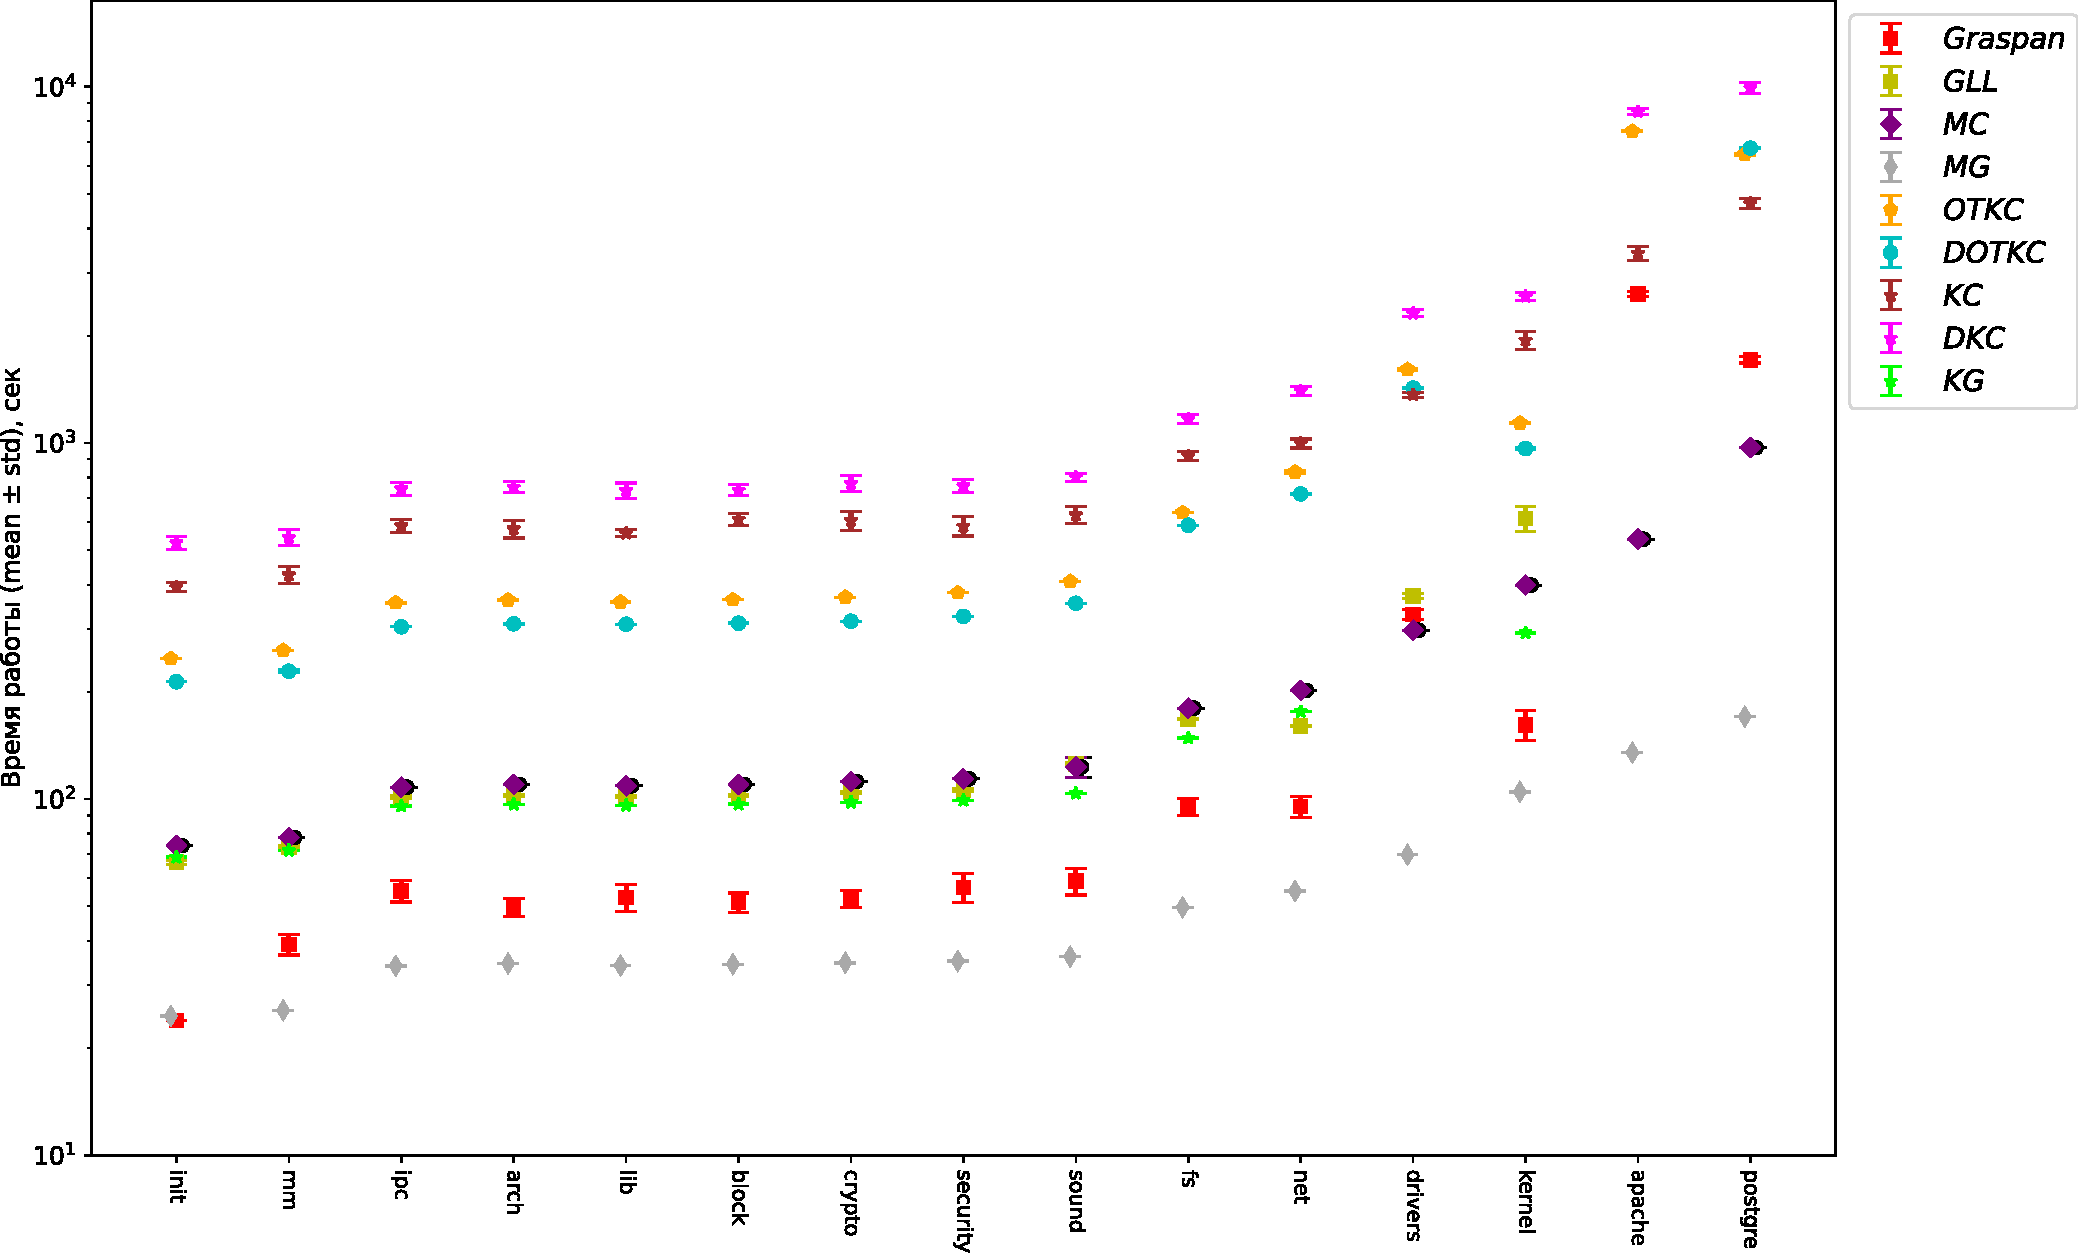
\includegraphics[width=\linewidth, height=8.1cm]{figures/ma_time.pdf}
        \caption{Время работы}
        \label{fig:ma_result_time}
    \end{subfigure}
    \begin{subfigure}{\textwidth}
        \centering
        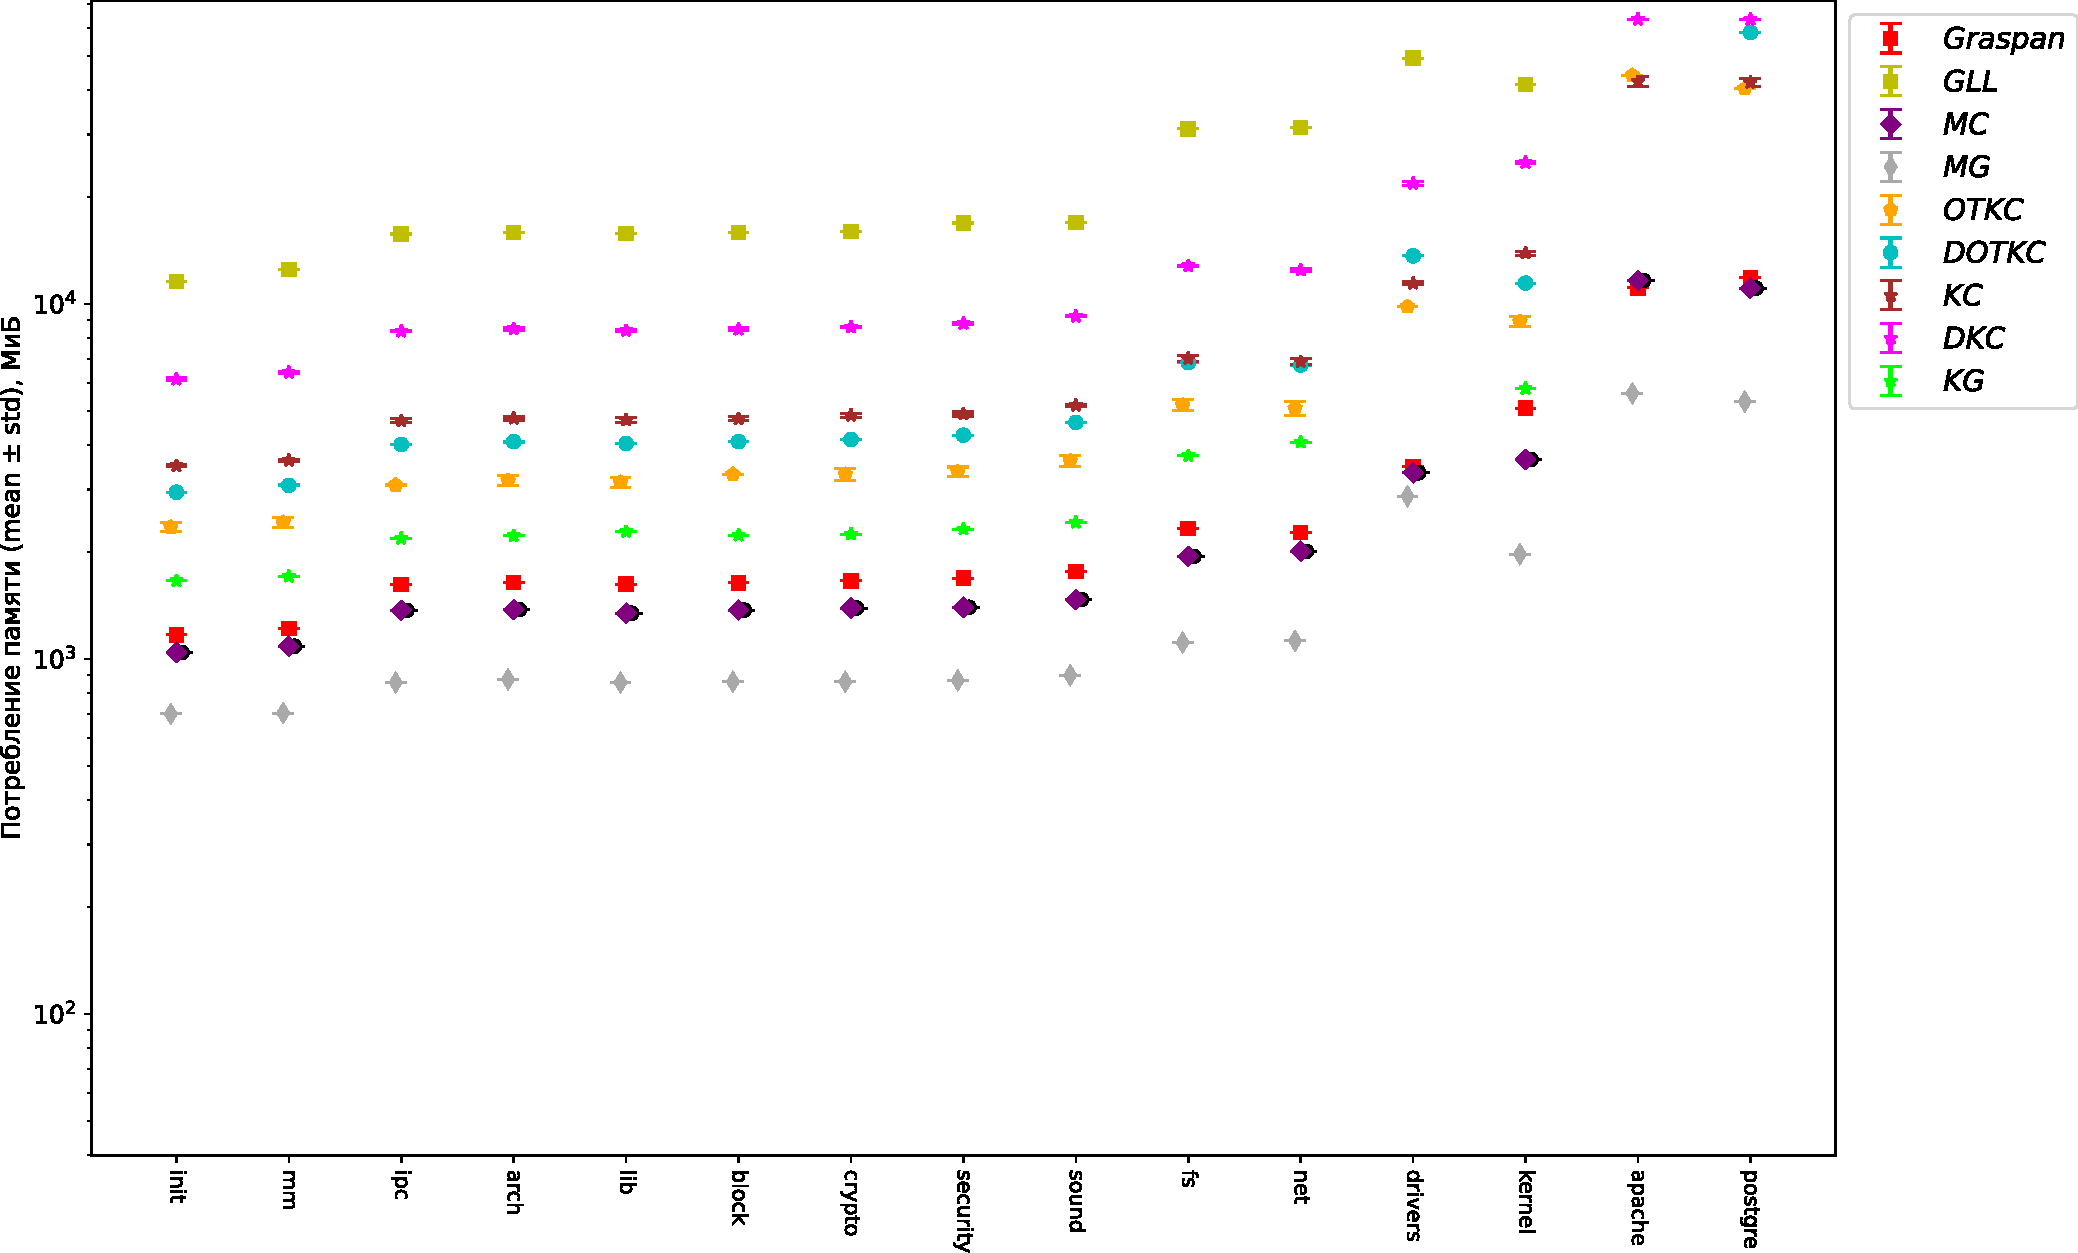
\includegraphics[width=\linewidth, height=8.1cm]{figures/ma_mem.pdf}
        \caption{Потребление памяти}
        \label{fig:ma_result_mem}
    \end{subfigure}
    \caption{Результаты для анализа псевдонимов}
    \label{fig:ma_result}
\end{figure}

\begin{figure}[h!]
    \begin{subfigure}{\textwidth}
        \centering
        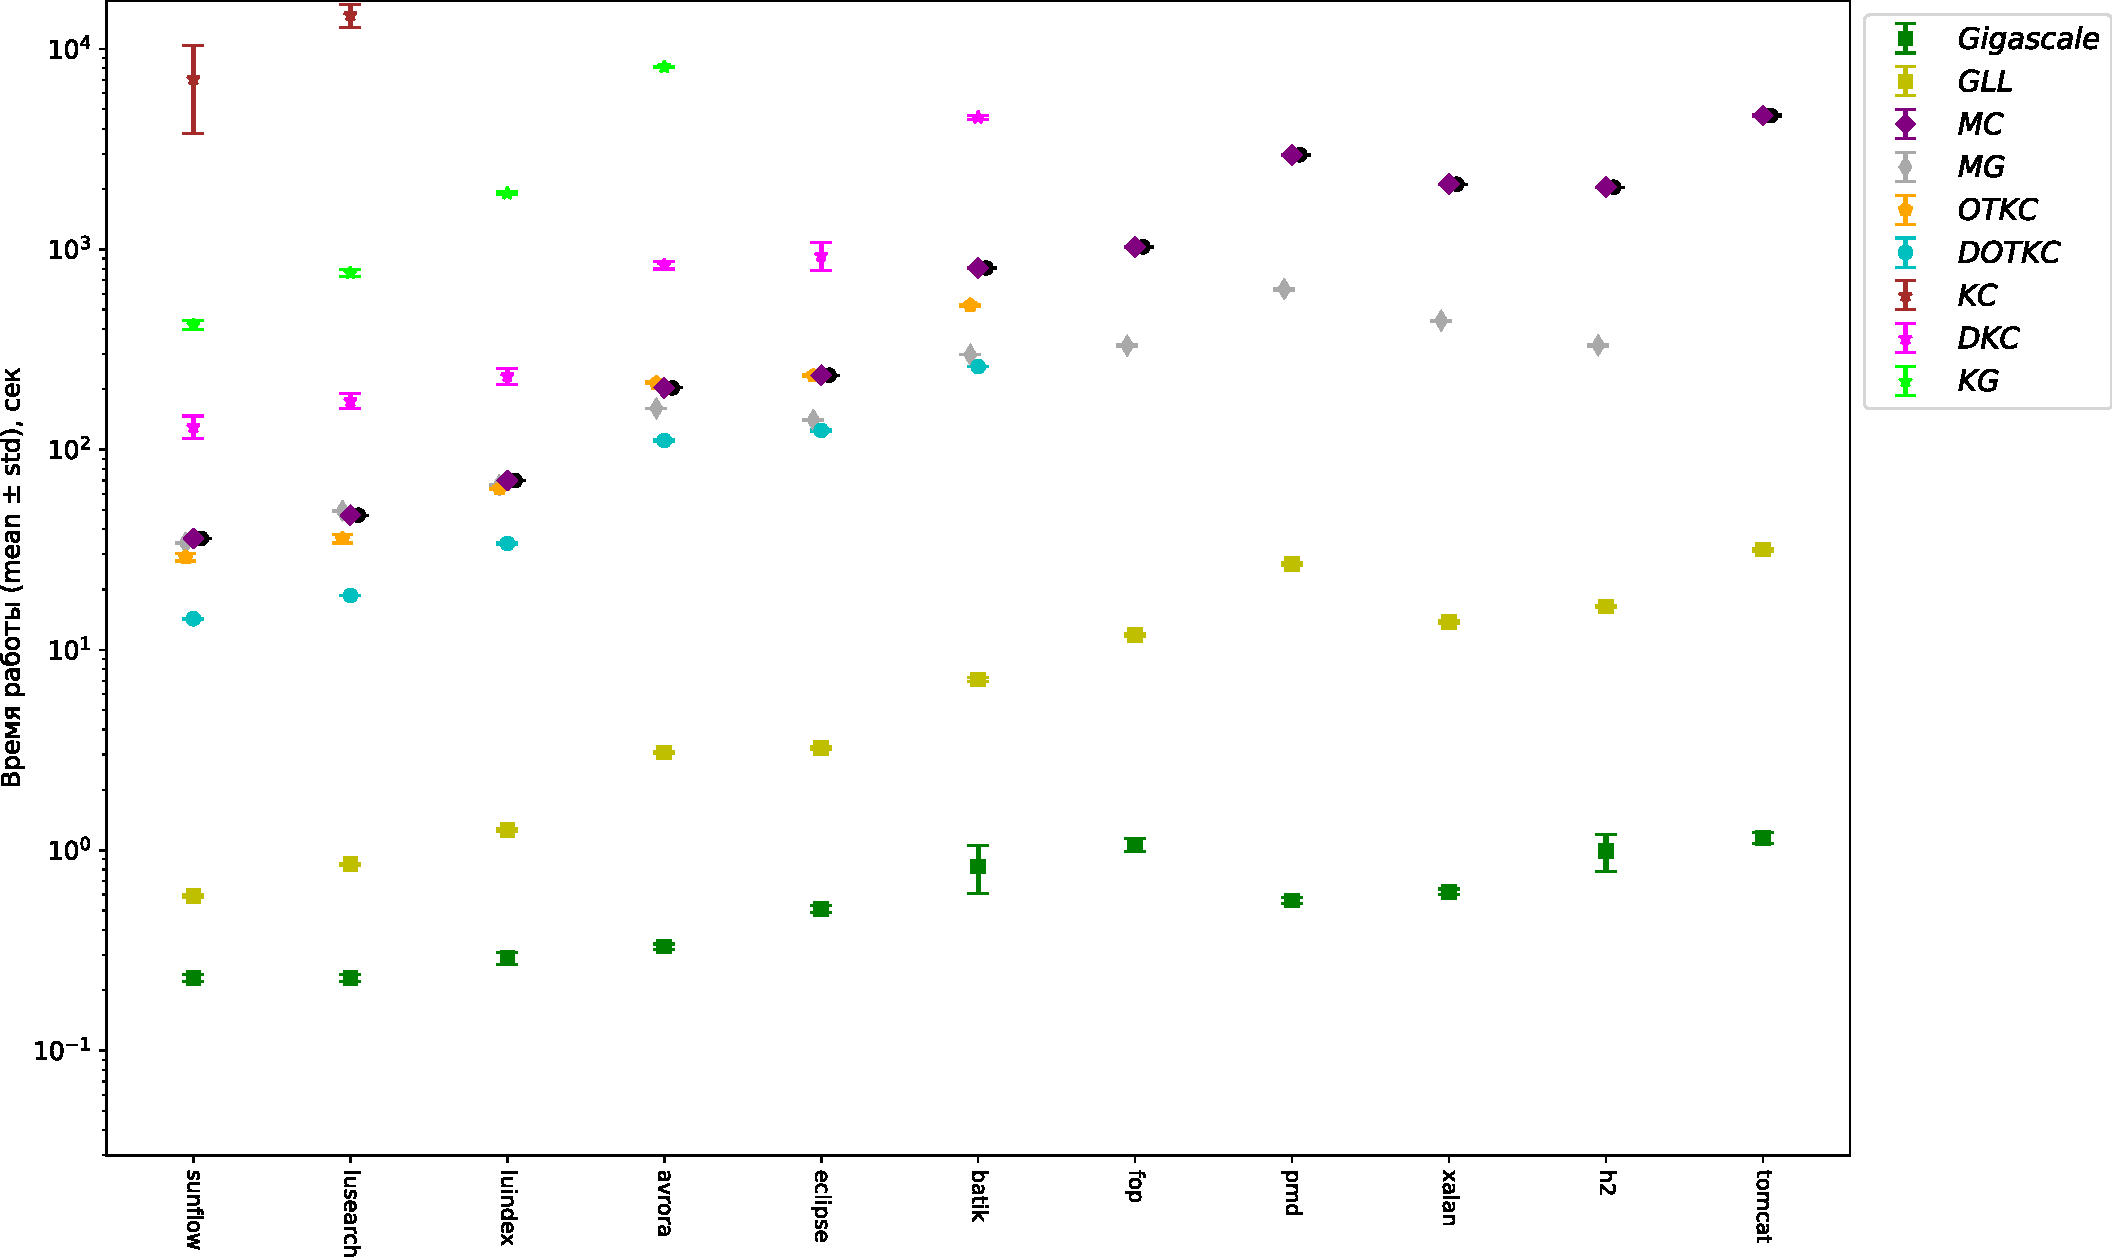
\includegraphics[width=\linewidth, height=8cm]{figures/java_time.pdf}
        \caption{Время работы}
        \label{fig:java_result_time}
    \end{subfigure}
    \begin{subfigure}{\textwidth}
        \centering
        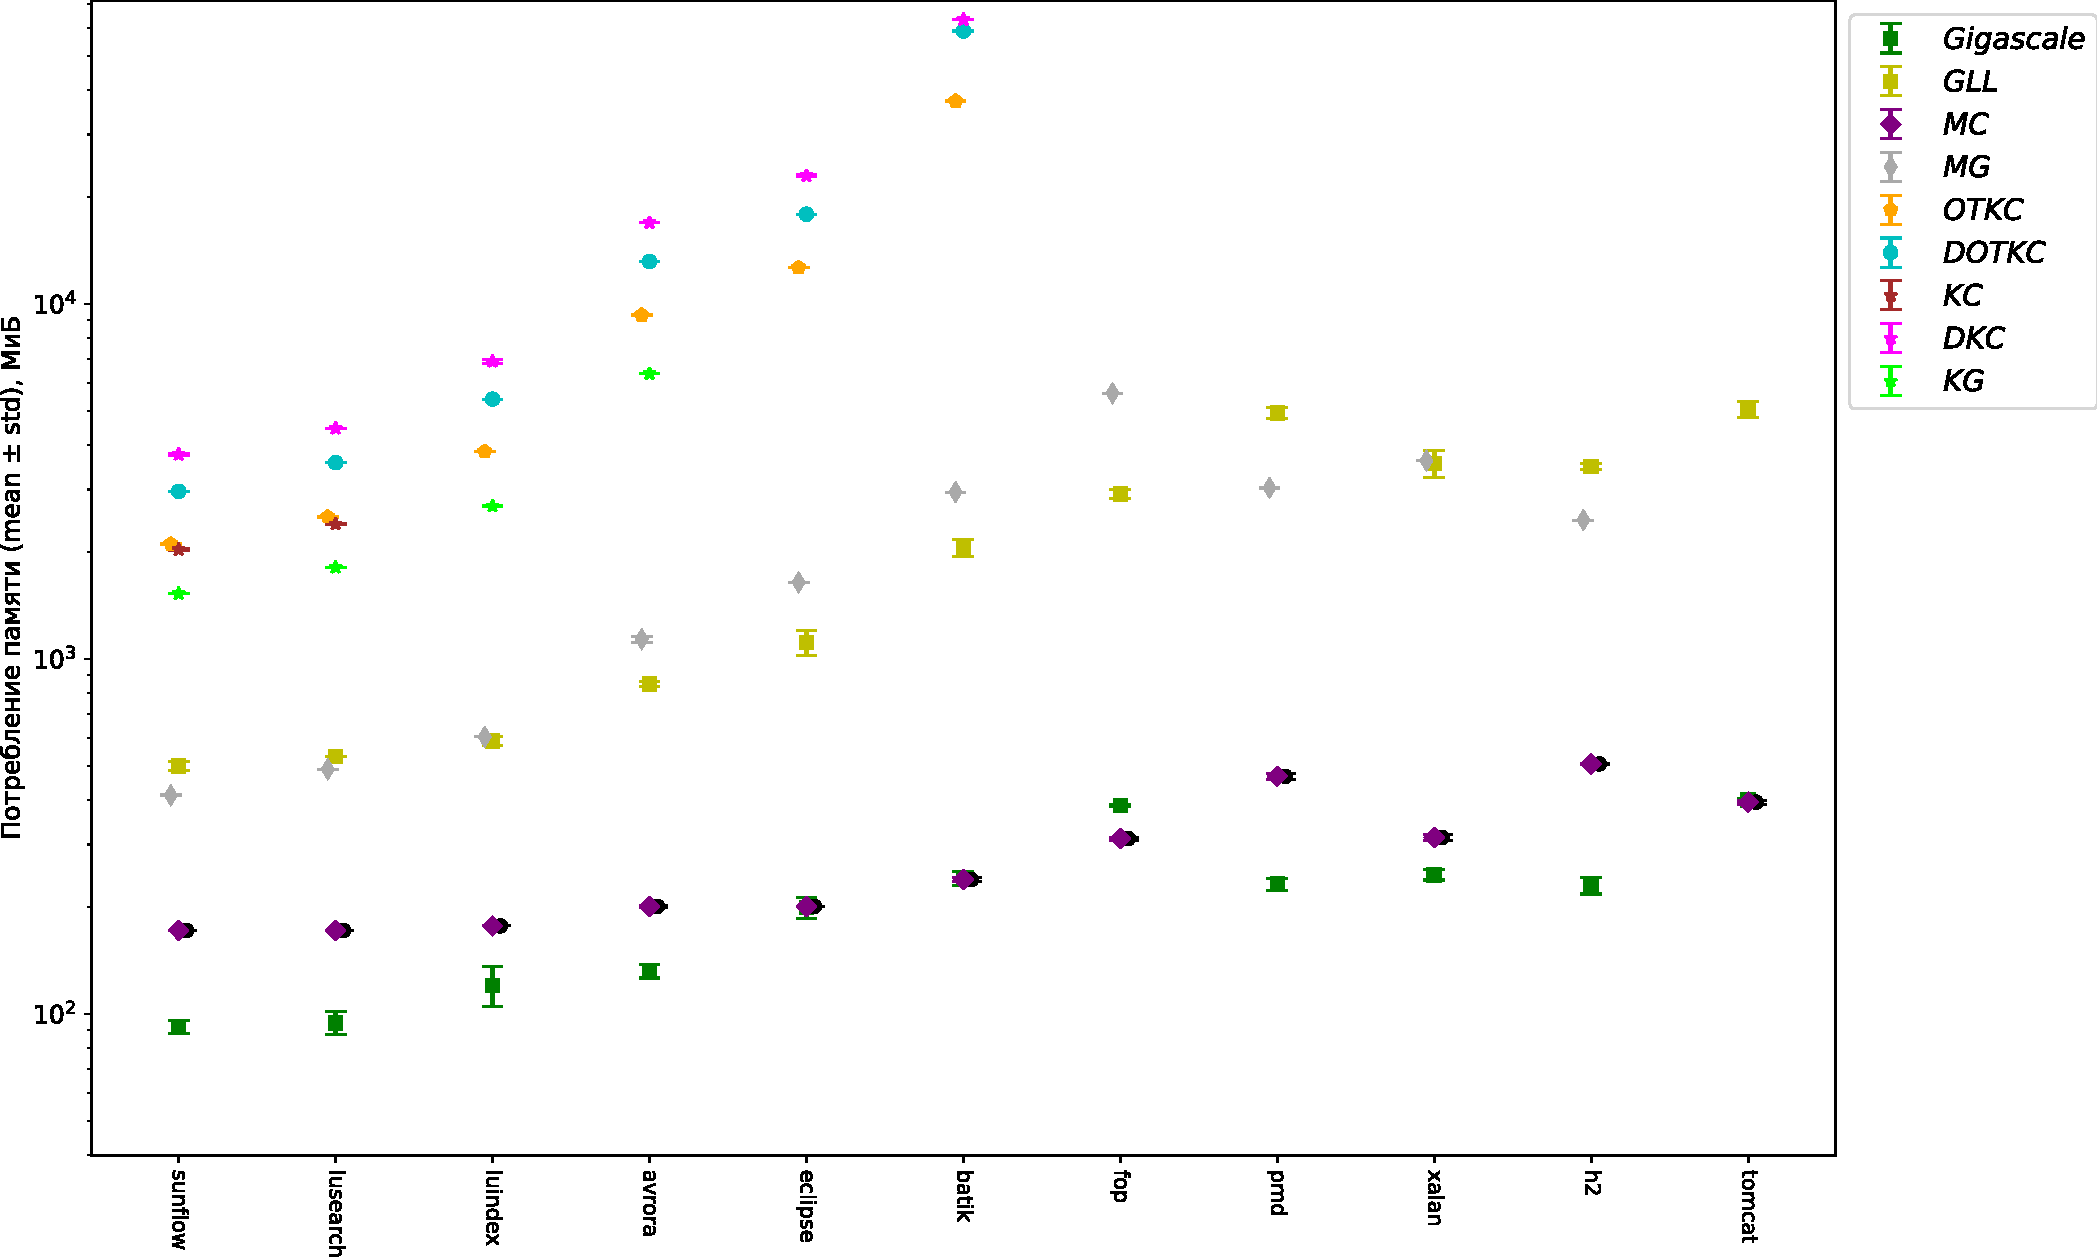
\includegraphics[width=\linewidth, height=8cm]{figures/java_mem.pdf}
        \caption{Потребление памяти}
        \label{fig:java_result_mem}
    \end{subfigure}
    \caption{Результаты для Points-to анализа, учитывающего поля}
    \label{fig:java_result}
\end{figure}

На основе полученных в результате экспериментов данных можно сделать следующие выводы.

\begin{itemize}
    \item При анализе псевдонимов наилучшие результаты (как время работы, так и потребление памяти) показала реализация матричного алгоритма для GPU. Для CPU же наименьшее время работы продемонстрировал Graspan. Однако при наличии в ответе большого числа пар достижимых вершин он работает значительно медленнее реализаций матричного алгоритма.
    \item Наименьшие время работы и потребление памяти при Points-to анализе, учитывающем поля, показала реализация Gigascale, работающая значительно быстрее всех остальных реализаций, что вполне обоснованно, ведь данный инструмент был разработан именно для такого анализа.
    \item Предложенные в работе модификация тензорного алгоритма и её инкрементальная версия работают быстрее других реализаций алгоритма для CPU в обоих видах анализа. Также можно отметить, что на небольших графах для Points-to анализа, учитывающего поля, инкрементальная версия продемонстрировала наименьшее время работы среди всех алгоритмов, основанных на операциях линейной алгебры. Однако эта реализация, как и базовый тензорный алгоритм, обладает таким недостатком, как большое потребление памяти. Это связано с большим размером получаемой в результате произведения Кронекера матрицы, который зависит и от размеров графа, и от размеров грамматики, что привело к ошибке нехватки памяти на графах fop, pmd, xalan, h2 и tomcat.
\end{itemize}

